\documentclass[runningheads,letterpaper]{llncs}

%%% PACKAGES %%%
%\usepackage[breaklinks]{hyperref}
%\usepackage{relsize}
%\usepackage{wrapfig}
%\usepackage{alltt}
%\usepackage{mathptmx}
%\usepackage[scaled]{helvet} % see www.ctan.org/get/macros/latex/required/psnfss/psnfss2e.pdf
%\DeclareMathAlphabet{\mathsf}{OT1}{phv}{m}{n}
%\usepackage{textpos}
%\usepackage{url}  % particularly useful for URLs in bib entries
\usepackage[breaklinks,draft=false]{hyperref}   % http://tex.stackexchange.com/questions/1522/pdfendlink-ended-up-in-different-nesting-level-than-pdfstartlink

% figures and graphics
%\usepackage{fancyref}
\usepackage{graphicx}
\usepackage{epstopdf}
\usepackage{subfigure}
%\usepackage{float,rotating}

% spacing
%\usepackage{relsize}
%\usepackage{setspace}
%\usepackage{xspace}
\usepackage{xcolor}
%\usepackage{booktabs}

\usepackage{listings}
%\usepackage{flushend}

\renewcommand{\floatpagefraction}{.8}%

% Define the style for OpenSHMEM programs
\renewcommand{\ttdefault}{pcr}
\lstdefinestyle{oshmem}{language=C,
                       keywordstyle=\bfseries, %\color{blue},
                       mathescape=true,
                       basicstyle=\ttfamily\scriptsize,
                       keepspaces=true,
                       morekeywords={auto},
                       otherkeywords={shmem_ctx_t,size_t}}

% Make OpenSHMEM the default style
\lstset{style=oshmem}

%%% AUTHORS %%%

%\newcommand{\kumar}{Kumar et al.\xspace}

\newcommand{\comment}[2]{\begin{quote}\textsf{\bf #1:} #2\end{quote}}
\newcommand{\fix}[1]{\textcolor{red}{#1}}

%%% SYTEMS %%%

\newcommand{\umpi}{UTS\_MPI\xspace}
\newcommand{\uupc}{UTS\_UPC\xspace}
\newcommand{\baseline}{BaselineWS\xspace}
\newcommand{\modified}{SuccessOnlyWS\xspace}
\newcommand{\wlOne}{T1WL\xspace}
\newcommand{\wlTwo}{T3WL\xspace}
\newcommand{\hcupcdef}{HabaneroUPC++ (default)\xspace}
\newcommand{\hcupcnew}{HabaneroUPC++ (parallel steals)\xspace}
\newcommand{\mpi}{MPI\xspace}
\newcommand{\upc}{UPC\xspace}
\newcommand{\outd}{out\_deque\xspace}
\newcommand{\ind}{in\_deque\xspace}
\newcommand{\ocr}{OCR\xspace}
\newcommand{\hcupc}{HabaneroUPC++\xspace}
\newcommand{\hcpp}{Habanero-C++\xspace}
\newcommand{\cpus}{6K\xspace}
\newcommand{\gnet}{GASNet\xspace}
\newcommand{\hcmpi}{HCMPI\xspace}
\newcommand{\hclib}{HClib\xspace}
\newcommand{\hci}{Habanero-C\xspace}
\newcommand{\hc}{Habanero\xspace}
\newcommand{\hj}{Habanero-Java\xspace}
\newcommand{\omp}{OpenMP\xspace}
\newcommand{\cppl}{C++11\xspace}
\newcommand{\cpp}{C++\xspace}
\newcommand{\upcp}{UPC++\xspace}
\newcommand{\xten}{X10\xspace}
\newcommand{\cilkp}{Cilk++\xspace}
\newcommand{\cilk}{Cilk\xspace}
\newcommand{\finish}{\textjava{finish}\xspace}
\newcommand{\fspmd}{\textjava{finish_spmd}\xspace}
\newcommand{\place}{\textjava{place}\xspace}
\newcommand{\places}{places\xspace}
\newcommand{\fasync}{\textjava{forasync}\xspace}
\newcommand{\async}{\textjava{async}\xspace}
\newcommand{\aany}{\textjava{asyncAny}\xspace}
\newcommand{\upcadvance}{\textjava{upcxx::advance}\xspace}
\newcommand{\upcasync}{\textjava{upcxx::async}\xspace}
\newcommand{\asyncat}{\textjava{asyncAt}\xspace}
\newcommand{\acopy}{\textjava{asyncCopy}\xspace}
\newcommand{\true}{\textjava{true}\xspace}
\newcommand{\false}{\textjava{false}\xspace}
\newcommand{\upccopy}{\textjava{upcxx::async_copy}\xspace}
\newcommand{\upcwait}{\textjava{upcxx::async_wait}\xspace}
\newcommand{\aawait}{\textjava{asyncAwait}\xspace}
\newcommand{\aphased}{\textjava{asyncPhased}\xspace}
\newcommand{\isolated}{\textjava{isolated}\xspace}
\newcommand{\when}{\textjava{when}\xspace}
\newcommand{\klass}{\textjava{class}\xspace}
\newcommand{\xatomic}{\textjava{atomic}\xspace}

%%% BENCHMARKS %%%

\newcommand{\lulesh}{\textbmx{LULESH}\xspace}
\newcommand{\ssort}{\textbmx{SampleSort}\xspace}

%%% PAGE NUMBERS %%%

\newcommand{\page}[1]{Section~\ref{#1}, page~\pageref{#1}}
\newcommand{\pageb}[1]{Section~\ref{#1} (page~\pageref{#1})}

%%% FONT %%%

\newcommand*{\textbmx}[1]{#1}  % No Sanserif in ACM SIG style file
%\newcommand*{\textbmx}[1]{\textsf{#1}}
\newcommand*{\textbm}[1]{\textbmx{#1}\xspace}
\newcommand{\cc}[1]{{\tt #1}}

\newcommand{\RemoveSpaces}[1]{%
  \begingroup
  \spaceskip=1sp
  \xspaceskip=1sp
  #1%
  \endgroup}

%%% FIX INFO %%%

%%% hyperreferences %%%

\newcommand{\doi}[1]{doi:~\href{http://dx.doi.org/#1}{\Hurl{#1}}}

%
% abbreviations
%

\newcommand{\eg}{e.g., }
\newcommand{\ie}{i.e., }
\newcommand{\etal}{et al. }

%
% Trademarks
%

\newcommand{\othertm}{\textsuperscript{$\star$}}
\newcommand{\regtm}{\textsuperscript{\textregistered{}}}
\newcommand{\tm}{{\scriptsize\texttrademark{}}}

%%%%%%%%%%%%%%%%%%%%%%%%%%%%%%%%%%%%%%%%%%%%%%%%%%%%%%%%%%%%%%%%%%%%%
% Stuff for pretty printing the source code using listings.sty
%

\lstloadlanguages{java}
\lstset{
  %numbers=left,
  numberstyle=\tiny\sffamily,
  stepnumber=1,
  numbersep=1em,
  language=java,                         % the language
  basicstyle=\scriptsize\ttfamily,     % the basic font family to use
  commentstyle=\scriptsize\it\ttfamily,% the font for comments
  stringstyle=\ttfamily,
  escapechar={\$},
  morekeywords={advance, event, forasync, finish_spmd, asyncAny, upcxx, asyncCopy, asyncAt, asyncAwait, asyncPhased, Address, Word, Offset, Extent, async, finish, def, val, fork, join}
}

% This command allows us to conviniently put java text inline.
%\newcommand{\textjava}[1]{{\lstset{basicstyle=\ttfamily}\lstinline@#1@}}
\DeclareRobustCommand{\textjava}[1]{{\lstset{basicstyle=\ttfamily}\lstinline@#1@}}
\newcommand{\cnull}{\textjava{NULL}\xspace}

%%%%%%%%%%%%%%%%%%%%%%%%%%%%%%%%%%%%%%%%%%%%%%%%%%%%%%%%%%%%%%%%%%%%%%%
%%%%%%%%%%%%%%%%%%%%%%%%%%%%%%%%%%%%%%%%%%%%%%%%%%%%%%%%%%%%%%%%%%%%%%%
%%%%%%%%%%%%%%%%%%%%%%%%%%%%%%%%%%%%%%%%%%%%%%%%%%%%%%%%%%%%%%%%%%%%%%%

%%% End:


\begin{document}
% \sloppy

\title{HOOVER}
\titlerunning{OpenSHMEM Contexts Using OFI Libfabric}

\author{Max Grossman\inst{1} \and
    Howard Pritchard\inst{2} \and
    Tony Curtis\inst{3} \and
    Vivek Sarkar\inst{4}
}

\authorrunning{Grossman et al.}

\institute{
    Rice University (\email{max.grossman@rice.edu}) \and Los Alamos National Laboratory
    \and
    Stony Brook University \and Georgia Institute of Technology
}

\maketitle

\renewcommand{\baselinestretch}{0.85}
Foo

\section{High-Level Usage}

HOOVER exposes a C/C++ API  to a SPMD programming model, inherited from the
OpenSHMEM programming model that it is built on top of. While most of the
application code does not need to be aware of the SPMD-ness of the underlying
runtime, application initialization is performed in parallel across all PEs in the
simulation. This choice was made deliberately so that large datasets could be
loaded across all PEs, rather than exposing sequential semantics by only
loading the dataset on a single PE and then broadcasting it.

The core data structure of HOOVER is a graph vertex. In HOOVER, a vertex can
have zero or more attributes attached to it, stored as a sparse
vector. During the execution of a HOOVER simulation, the user-level, application-specific
code is primarily responsible for reading and updating attributes
on local and remote vertices based on application-specific semantics.

Attributes in HOOVER are split into two categories: positional and logical.
Positional attributes on a vertex define its relationship and distance to other
vertices in the simulation. Positional attributes are used by HOOVER to
automatically update edges between vertices as they move ``closer'' or ``farther'' away.
For example, positional attributes might be the physical location of a
vertex in a 2D or 3D space, defining its location relative to other vertices.
Logical attributes are additional vertex attributes used by the
programmer for application-specific information, but which are not used by the
HOOVER runtime system.

At a high level, a HOOVER program starts with the user configuring a graph
problem by defining the initial state/attributes of all vertices in it. This
initial state is then passed into the HOOVER runtime along with several
application-specific callbacks. All future execution is then coordinated by the
HOOVER runtime, with application callbacks made when application-specific
behavior or updates are needed.

\begin{figure}
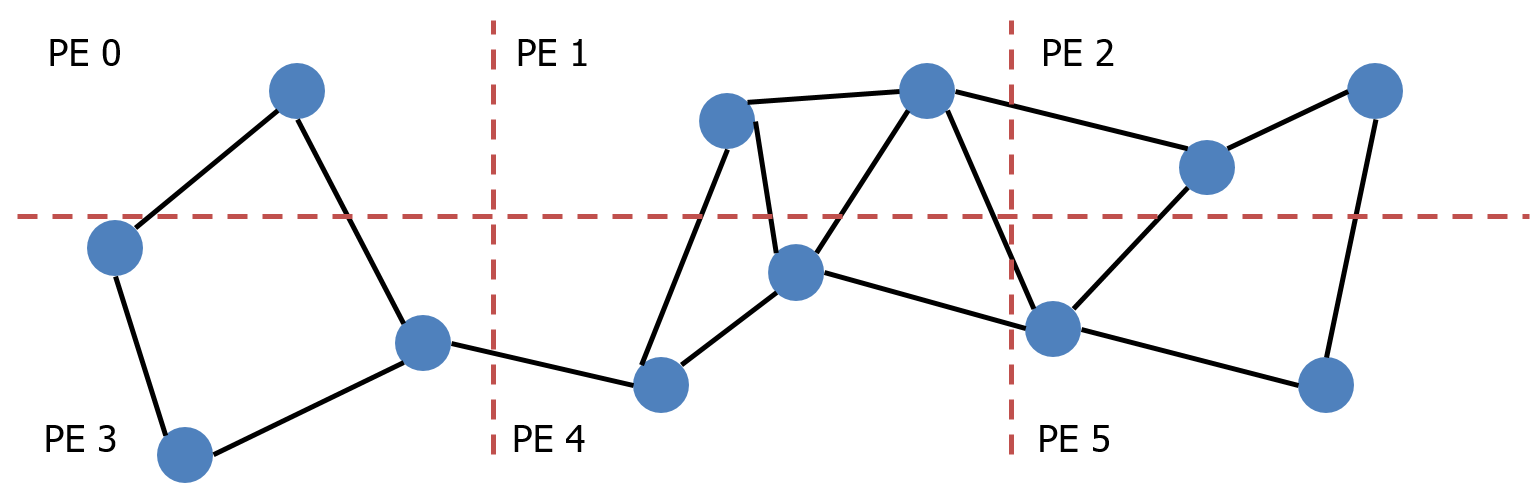
\includegraphics[width=\columnwidth]{pe_diag.png}
\caption{Illustration of a HOOVER graph distributed across PEs with cross-PE
    edges.}
\label{fig:pe_diag}
\end{figure}

\subsection{Target Application Pattern}

While HOOVER is a general dynamic graph processing, simulation, and analytics
framework it also offers specialized capabilities for a particular class of
dynamic graph problems. The classical HOOVER problem follows the following high
level execution flow:

\begin{enumerate}
    \item The application defines a large number of vertices partitioned across
        PEs, as well as callbacks to update their state (among other things).
    \item The HOOVER framework begins iterative modeling of vertex behavior
        through repeated callbacks to user-level functions, evolving vertex
        state over time. All PEs execute entirely de-coupled from each other.
        While each PE is asynchronously made aware of summaries of the state
        change in other PEs, no PE is ever blocked on or performing two-sided
        communication with any other PE.
    \item After some time, two or more PEs discover they are related. This
        ``relationship'' is entirely user-directed and in the control of user
        callbacks. After this connectivity is discovered, those PEs will enter
        lockstep execution with each other and share data on each timestep.
        Multiple clusters of coupled PEs may evolve over time, with separate
        groups of PEs becoming interconnected or all PEs evolving into a single,
        massive cluster depending on the application.
    \item Eventually, application termination is either signalled by a PE or
        controlled by all PEs reaching a maximum number of timesteps.
\end{enumerate}

At this point, an illustrative example might be useful: malware spread over
Bluetooth. Malware propagation modeling can be expressed as a graph problem,
where vertices in the graph represent Bluetooth devices and edges represent direct
connectivity between two devices. Executing malware propagation on the
HOOVER framework might look something like:

\begin{enumerate}
    \item The application developer would define the actors in the simulation as
        vertices passed down to the HOOVER framework. Each actor would represent
        a device, and may include attributes such as the range of its Bluetooth
        hardware, the model its Bluetooth hardware, the speed at which it can
        move, or its initial infected/uninfected status.
    \item HOOVER would then begin execution, updating device infection status,
        position, and connectivity with other devices based on user callbacks and
        other information passed in by the application developer. As iterations
        progress, more and more devices might become infected from a small
        initial seed of infected devices.
    \item Eventually, two or more PEs may become coupled at the application
        developer's direction. For example, the developer might instruct two PEs
        to become coupled if a device resident on one PE infects a device resident
        on another. By entering coupled, lockstep execution those two PEs can
        now compute several joint metrics about the infection cluster they
        collectively store, such as number of infected devices or rate of
        infection progression. Note that even when PEs create a tightly coupled
        cluster, they still interact as usual with any other PEs in the
        simulation which they are not coupled with.
\end{enumerate}

\section{API}

\subsection{Vertex APIs}

The core data structure of HOOVER is the graph vertex, represented by objects of
type \texttt{hvr\_sparse\_vec\_t}. Application developers are not expected to
manipulate the internal state of this object directly, but rather using the
following APIs.

Below, several terms may be used to refer to a simulation vertex, including
vertex, sparse vector, or actor.

\subsubsection{\texttt{hvr\_sparse\_vec\_create\_n}}

\begin{verbatim}
hvr_sparse_vec_t *hvr_sparse_vec_create_n(
        const size_t nvecs);
\end{verbatim}

Create \texttt{nvecs} sparse vectors/vertices. This API must be called
collectively on all PEs with the same value of \texttt{nvecs} on each PE. This
will return initialized but empty vertices to the user, to be populated with
initial information.

\subsubsection{\texttt{hvr\_sparse\_vec\_set\_id}}

\begin{verbatim}
void hvr_sparse_vec_set_id(const vertex_id_t id,
        hvr_sparse_vec_t *vec);
\end{verbatim}

Set a globally unique ID \texttt{id} for vertex \texttt{vec} in the current
simulation. It is the programmer's responsibility to provide each vertex a
globally unique ID, and the runtime performs no checks to verify the uniqueness
of each ID. This API must be called once for each vertex in a given simulation
before launching the simulation with the \texttt{hvr\_body} API (described
below).

Vertex IDs do not need to follow any pattern or be contiguous, but application
developers are advised to assign their vertex IDs in such a way that looking up
the PE for a given vertex is a quick, efficient, and preferrably constant time
operation.

\subsubsection{\texttt{hvr\_sparse\_vec\_get\_id}}

\begin{verbatim}
vertex_id_t hvr_sparse_vec_get_id(hvr_sparse_vec_t *vec);
\end{verbatim}

Fetch the globally unique ID assigned to the passed vertex.

\subsubsection{\texttt{hvr\_sparse\_vec\_get\_owning\_pe}}

\begin{verbatim}
int hvr_sparse_vec_get_owning_pe(hvr_sparse_vec_t *vec);
\end{verbatim}

Fetch the PE that owns the passed vertex, i.e. the PE that created and
initialized it. Information on PE ownership is automatically maintained by the
HOOVER runtime. No dynamic load balancing of vertices is performed in HOOVER,
and so vertex ownership is a static and one-to-one relationship.

\subsubsection{\texttt{hvr\_sparse\_vec\_set}}

\begin{verbatim}
void hvr_sparse_vec_set(const unsigned feature,
        const double val, hvr_sparse_vec_t *vec,
        hvr_ctx_t in_ctx);
\end{verbatim}

Set the vertex attribute identified by \texttt{feature} to store the value
\texttt{val} in the vertex \texttt{vec}.

\subsubsection{\texttt{hvr\_sparse\_vec\_get}}

\begin{verbatim}
double hvr_sparse_vec_get(const unsigned feature,
        hvr_sparse_vec_t *vec, hvr_ctx_t in_ctx);
\end{verbatim}

Fetch the value stored for attribute \texttt{feature} in vertex \texttt{vec}. If
the specified attribute was never set on this vertex, the default behavior is to
abort the current simulation.

\subsubsection{\texttt{hvr\_sparse\_vec\_dump}}

\begin{verbatim}
void hvr_sparse_vec_dump(hvr_sparse_vec_t *vec, char *buf,
        const size_t buf_size, hvr_ctx_t in_ctx);
\end{verbatim}

A utility function for creating a human-readable string for the passed vertex
into the provided character \texttt{buf}, which is at least of length
\texttt{buf\_size} bytes. This API can be useful for debugging or other user
diagnostics.

\subsection{Core APIS}

The core of HOOVER is encapsulated in four APIS.

\subsubsection{\texttt{hvr\_ctx\_create}}

\begin{verbatim}
extern void hvr_ctx_create(hvr_ctx_t *out_ctx);
\end{verbatim}

\texttt{hvr\_ctx\_create} initializes the state of a user-allocated HOOVER
context object to be used in later HOOVER user and runtime operations. This API
does not allocate space for the context, the \texttt{out\_ctx} parameter is
expected to point to at least \texttt{sizeof(hvr\_ctx\_t)} bytes of valid
memory. \texttt{out\_ctx} may be on the stack or heap memory segment.

The HOOVER context is used to store several pieces of global state for a given HOOVER
simulation, such as a pointer to the local vertices in the simulation being
managed by the current PE. This should be considered an opaque object by any
application developers, and internal context state should not be directly
manipulated.

HOOVER assumes that the user has already called \texttt{shmem\_init} to
initialize the OpenSHMEM runtime before calling \texttt{hvr\_ctx\_create}.

\subsubsection{\texttt{hvr\_init}}

\begin{verbatim}
extern void hvr_init(const uint16_t n_partitions,
        const vertex_id_t n_local_vertices,
        hvr_sparse_vec_t *vertices,
        hvr_update_metadata_func update_metadata,
        hvr_might_interact_func might_interact,
        hvr_check_abort_func check_abort,
        hvr_vertex_owner_func vertex_owner,
        hvr_actor_to_partition actor_to_partition,
        const double connectivity_threshold,
        const unsigned min_spatial_feature_inclusive,
        const unsigned max_spatial_feature_inclusive,
        const hvr_time_t max_timestep, hvr_ctx_t ctx);
\end{verbatim}

\texttt{hvr\_init} completes initialization of the HOOVER context object by
populating it with several pieces of user-provided information (e.g. callbacks)
and allocating internal data structures. \texttt{hvr\_init} does not launch the
simulation itself, but is the last step before doing so. The arguments passed
are described below:

\begin{enumerate}
    \item \texttt{n\_partitions} - During execution, HOOVER divides the
        simulation space up into partitions as directed by the
        \texttt{actor\_to\_partition} callback (described below). These
        partitions are used to approximately detect interactions between actors
        by first finding actor-to-partition interaction. This is similar but not
        identical to techniques used in the Fast Multipole Method. This argument
        specifies the number of partitions the application developer will use.
    \item \texttt{n\_local\_vertices} - The number of vertices managed by the
        local PE.
    \item \texttt{vertices} - The vertices managed by the local PE. This array
        should be allocated using \texttt{hvr\_sparse\_vec\_create\_n}, and each
        vertex in it should have been initialized using
        \texttt{hvr\_sparse\_vec\_set\_id} and \texttt{hvr\_sparse\_vec\_set}.
    \item \texttt{update\_metadata} - A user callback. On each timestep,
        \texttt{update\_metadata} is passed each local vertex one-by-one along
        with all vertices that the current vertex has edges with (including
        remote vertices). update\_metadata is responsible for updating the local
        state of the current vertex, and deciding if based on those updates any
        remote PEs should become coupled with the current PE's execution.
    \item \texttt{might\_interact} - A user callback. \texttt{might\_interact}
        is called with a single partition ID and a set of partitions to
        determine if a vertex in the provided partition may interact with any
        actor in any partition in the passed set.
    \item \texttt{check\_abort} - A user callback. \texttt{check\_abort}
        is used by the application developer to determine if the current
        simulation should exit based on the state of all local vertices
        following a full timestep. \texttt{check\_abort} also computes any
        local metrics, which are then shared with coupled PEs to compute coupled
        metrics.
    \item \texttt{vertex\_owner} - A user callback. Given a globally unique
        vertex ID, the user is expected to return the PE owning that vertex and
        the offset in that PE's vertices of the specified vertex.
    \item \texttt{actor\_to\_partition} - A user callback. Given a vertex,
        return the partition it belongs in.
    \item \texttt{connectivity\_threshold}, \\
        \texttt{min\_spatial\_feature\_inclusive}, \\
        \texttt{max\_spatial\_feature\_inclusive} - These arguments are all used
        to update edges. Recall that HOOVER automatically updates inter-vertex
        edges based on their ``nearness'' to other vertices in the simulation,
        by some distance measure. Today, that is simply an N-dimensional
        Euclidean distance measure on the features in the range
        [\texttt{min\_spatial\_feature\_inclusive},
        \texttt{max\_spatial\_feature\_inclusive}]. If the computed distance is
        less than \texttt{connectivity\_threshold} those vertices have an edge
        created between them.
    \item \texttt{max\_timestep} - A limit on the number of timesteps for HOOVER
        to run.
    \item \texttt{ctx} - The HOOVER context to initialize. This ctx should
        already have been zeroed using \texttt{hvr\_ctx\_create}.
\end{enumerate}

\subsubsection{\texttt{hvr\_body}}

\begin{verbatim}
extern void hvr_body(hvr_ctx_t ctx);
\end{verbatim}

Launch the simulation problem, as specified by the provided \texttt{ctx}.
\texttt{hvr\_body} only returns when the local PE has completed execution,
either by exceeding the maximum number of timesteps or through a non-zero return
code from the \texttt{check\_abort} callback.

\subsubsection{\texttt{hvr\_finalize}}

\begin{verbatim}
extern void hvr_finalize(hvr_ctx_t ctx);
\end{verbatim}

Perform cleanup of the simulation state. HOOVER assumes that
\texttt{shmem\_finalize} is called after \texttt{hvr\_finalize}.

\subsection{HOOVER Application Skeleton}

Given the above APIs, a standard HOOVER application has the following structure:

\begin{verbatim}
hvr_ctx_t ctx;
hvr_ctx_create(&ctx);

// Create and initialize the vertices in the simulation
hvr_sparse_vec_t *vertices = hvr_sparse_vec_create_n(...);
...

hvr_init(...);

// Launch the simulation
hvr_body(ctx);

// Analyze and display the results of the simulation
...

hvr_finalize(ctx);

\end{verbatim}

\section{Runtime}

With our understanding of the user-facing APIs for HOOVER, we can now discuss
how HOOVER operates on the backend. We will split this into two discussions: 1)
a description of the vertex/sparse vector data structure used, and 2) a
description of the various steps taken by the HOOVER runtime on each timestep of
an iterative simulation.

\subsection{Versioned Sparse Vectors}

While HOOVER sparse vectors expose simple read and modify APIs to the user, they
are subtely complex.

The root of this complexity is the decoupled nature of HOOVER's execution. For
scalability reasons, HOOVER was designed to avoid all two-sided, blocking, or
collective operations between any two de-coupled PEs. As such, any PE may
fetch vertex data from any other PE at any time during the simulation without
any involvement from the PE being accessed. As such, the sparse vector data
structure must be designed to be always consistent, such that remote accessors
can get information from it even if the owning PE is currently modifying it.

Additionally, because HOOVER is iterative it has some measure of progress, time,
and ordering between timesteps. Indeed, de-coupled PEs may have
reached very different timesteps in the simulation before their first
interaction. However, it would be undesirable for the slower PE to be able to
read data from the future on the faster PE - we would like any information
accessed to be mostly consistent for a given timestep (though perhaps not from
that precise timestep). As a result, it is necessary to have some history or
versioning built in to HOOVER's sparse vector data structure such that
de-coupled PEs on different timesteps can still fetch consistent data from each
other.

Hence, internally the sparse vector data structure stores its state going back
many timesteps. Additionally, when updating a sparse vector with new values,
those values are tagged with the current timestep. A simplified version of the
actual sparse vector declaration is shown below:

\begin{verbatim}
typedef struct _hvr_sparse_vec_t {
    // Globally unique ID for this node
    vertex_id_t id;

    // PE that owns this vertex
    int pe;

    // Values for each feature
    double values[HVR_BUCKETS][HVR_BUCKET_SIZE];

    // Feature IDs, all entries in each bucket guaranteed unique
    unsigned features[HVR_BUCKETS][HVR_BUCKET_SIZE];

    // Number of features present in each bucket
    unsigned bucket_size[HVR_BUCKETS];

    // Timestamp for each bucket
    hvr_time_t timestamps[HVR_BUCKETS];
} hvr_sparse_vec_t;
\end{verbatim}

Here, the key fields are \texttt{timestamps}, \texttt{bucket\_size},
\texttt{values}, and \texttt{features} each of which is a circular buffer. The
sparse vector above has the ability to store history for this sparse vector's
state going back \texttt{HVR\_BUCKETS} timesteps, with up to
\texttt{HVR\_BUCKET\_SIZE} features in the sparse vector.

Each time the first attribute is set on a new timestep, a bucket is allocated to
it by finding the oldest bucket. The most recent state of the sparse vector from
the most recent timestep is copied to the new bucket, including its
\texttt{features}, \texttt{values}, and \texttt{bucket\_size}. Then, additional
changes for the current timestep are made on top of those copied values.

Anytime a feature needs to be read from a sparse vector, a timestep to read the
value for is also passed in (either explicitly if from the HOOVER runtime or
implicitly using the calling PE's context). The bucket that is closest to that
timestep but not past it is then used to return the requested feature.

While this design is flexible and solves the problem of de-coupled data accesses
in a massively distributed system, it naturally comes with drawbacks. It is
relatively wasteful of memory, consuming many times the number of bytes than
what would be needed to simply store the current state of the sparse vector. Of
course, this also has implications for bytes transferred over the network. This
design also limits how out-of-sync two PEs can become as a result of using a
fixed-size circular buffer. If one PE becomes more than \texttt{HVR\_BUCKETS}
behind the other PE, it will no longer be able to fetch valid values from the
other's vertices.

\subsection{Core Runtime Execution Flow}



\section{Performance of an Example Use Case}

As an example, we use a simplified infectious disease modeling problem to
demonstrate and benchmark the current state of the HOOVER framework.

Our simple infectious disease model is expressed on a two-dimensional problem
space, which represents some geographic area. Partitions are created as a
regular, two-dimensional grid across the whole problem space.

Each actor in the problem is given 7 attributes:

\begin{enumerate}
    \item A two-component position.
    \item A two-component home location for this vertex.
    \item A two-component current destination location for this vertex.
    \item A single attribute indicating if a vertex is infected or uninfected.
\end{enumerate}

On each timestep, each actor does the following:

\begin{enumerate}
    \item If the current actor is still uninfected, it iterates over all
        vertices with which it shares edges and checks if any are infected. If
        any are infected, the current actor marks itself infected. If the actor
        which infects this actor comes from another PE, the current PE becomes
        coupled with the remote PE.
    \item The current actor then updates its current position based on its home
        location and its destination location. An actor's home location is some
        point in the 2D problem space which it never moves more than a certain
        distance from. A point's destination location is the current point in
        the 2D problem space that an actor is moving towards, which must be near
        its home location.
        \begin{enumerate}
            \item If the actor has not yet reached its destination location, it
                simply updates its current location to continue moving towards
                it.
            \item If the actor has reached its destination location, it
                computes a new destination location within some radius of its
                home and begins moving towards its new destination.
        \end{enumerate}
\end{enumerate}

Benchmarking scalability of irregular problems like those that the HOOVER
framework targets can be difficult, as even small changes in the scale of the
problem or compute resources available can drastically impact the communication
or computational patterns of the application.

Additionally, we would like to strongly emphasize that all performance results shown here
are works-in-progress and that this report will be frequently updated as scaling
improves. Performance bottlenecks and issues continue to be ironed
out of the HOOVER framework, and scalability improves on a weekly basis.
However, this report will serve as a useful document for tracking those
improvements.

Still, we try to use this example problem to illustrate the current scaling
characteristics of the HOOVER framework as several parameters and tunables are
changed.

These experiments are run on a small cluster at Los Alamos National Laboratory
consisting of SGI/HPE C1104-GP2 servers connected with Mellanox ConnectX5.
Each server has 2 sockets, each containing 8 hyperthreaded cores, and 64 GB of
memory. In the experiments below, we run with one PE per core (i.e. 8 PEs per
socket).

As performance continues to improve over time, this report will be updated with
those improvements. Table~\ref{tab:hoover_versions} maps from version numbers used in the text
below to commit hashes in the Github repo. In general, any figures/tables will
include in their caption which version of HOOVER the results are collected from.

\begin{table}
\centering
\begin{tabular}{ | l | l | l | }
\hline
\textbf{Version Number} & \textbf{Git Hash}                         & \textbf{Date} \\\hline
0.1                     & \texttt{385911bb27f74fd74a8f038f95a2447cda372ec4} & Feb 10 2018 \\\hline
0.2                     & \texttt{38591d9adf732c144ced382175348031f8518bad} & Feb 27 2018 \\\hline
0.3                     & \texttt{4f9350fcc2d624ae14cffde6aae08b63a7d3ad16} & Mar 02 2018 \\\hline
0.4                     & \texttt{0129e2a81c2a14959e8966965b25c3fc7cf5c752} & Mar 17 2018 \\\hline
0.5                     & \texttt{09631dfeb925adaccb52f63ff4eaad4ba4fc8243} & Apr 08 2018 \\\hline
0.6                     & \texttt{26deaf397ee98ca785bd381528047ef79790814c} & May 02 2018 \\\hline
\end{tabular}
\caption{Strong scaling of the HOOVER framework on OSSS OpenSHMEM running a
    simple infectious disease model with varying \# of iters and infection
    radius.}
\label{tab:hoover_versions}
\end{table}

These experiments are run with OSSS OpenSHMEM over UCX. HOOVER is compiled using
gcc 6.3.0 with -O2 optimization turned on.

\subsection{Strong Scaling}
\label{sec:strong_scaling}

These experiments test the strong scaling of HOOVER while varying two
simulation parameters but keeping the problem space fixed. We vary the number of
timesteps/iterations to run the simulation for, and the infection radius.
Infection radius controls how quickly the infection spreads from one actor to
another, and so an increased infection radius leads to more infected actors
across more PEs (and hence, more rapid PE coupling).
Tables~\ref{tab:strong_scaling1}, \ref{tab:strong_scaling2},
\ref{tab:strong_scaling3}, \ref{tab:strong_scaling4},
and~\ref{tab:strong_scaling5} show the results of these experiments.

\begin{table}
\centering
\begin{tabularx}{\textwidth}{ | l || X | X | X | X | X | X | }
\hline
\textbf{\# Iters}           & \multicolumn{2}{|X|}{\textbf{10}} & \multicolumn{2}{|X|}{\textbf{100}} & \multicolumn{2}{|X|}{\textbf{200}} \\\hline
\textbf{Infection Radius}   & 4.0          & 10.0         & 4.0           & 10.0          & 4.0           & 10.0 \\\hline
1 node                      & 22,360 & 29,299 & 239,527 & 298,234 & 459,211 & 676,952 \\\hline
4 nodes                     & 1,725  & 3,075  & 16,167  & 32,620  & 32,915  & 66,724 \\\hline
16 nodes                    & 4,389  & 2,916  & 31,517  & 50,068  & 60,293  & 115,186 \\\hline
\end{tabularx}
\caption{Strong scaling of the HOOVER framework v0.1 on OSSS OpenSHMEM running a
    simple infectious disease model with varying \# of iters and infection
    radius.}
\label{tab:strong_scaling1}
\end{table}

\begin{table}
\centering
\begin{tabularx}{\textwidth}{ | l || X | X | X | X | X | X | }
\hline
\textbf{\# Iters}           & \multicolumn{2}{|X|}{\textbf{10}} & \multicolumn{2}{|X|}{\textbf{100}} & \multicolumn{2}{|X|}{\textbf{200}} \\\hline
\textbf{Infection Radius}   & 4.0          & 10.0         & 4.0           & 10.0          & 4.0           & 10.0 \\\hline
1 node                      & 15,169        & 18,321        & 145,107        & 197,610        & 291,928        & 399,285 \\\hline
4 nodes                     & 1,813         & 2,804         & 13,043         & 22,007         & 25,785         & 44,847 \\\hline
16 nodes                    & 1,870         & 1,877         & 7,201          &  12,364        & 9,658          & 27,461 \\\hline
\end{tabularx}
\caption{Strong scaling of the HOOVER framework v0.2 on OSSS OpenSHMEM running a
    simple infectious disease model with varying \# of iters and infection
    radius.}
\label{tab:strong_scaling2}
\end{table}

\begin{table}
\centering
\begin{tabularx}{\textwidth}{ | l || X | X | X | X | X | X | }
\hline
\textbf{\# Iters}           & \multicolumn{2}{|X|}{\textbf{10}} & \multicolumn{2}{|X|}{\textbf{100}} & \multicolumn{2}{|X|}{\textbf{200}} \\\hline
\textbf{Infection Radius}   & 4.0          & 10.0         & 4.0           & 10.0          & 4.0           & 10.0 \\\hline
1 node                      & 12,919 & 18,139 & 142,675 & 193,895 & 303,930 & 401,899 \\\hline
4 nodes                     &  1,817 &  3,043 &  12,321 &  22,917 &  24,266 &  42,755 \\\hline
16 nodes                    &   340 &   657 &   3,204 &  12,166 &   6,996 &  28,947 \\\hline
\end{tabularx}
\caption{Strong scaling of the HOOVER framework v0.3 on OSSS OpenSHMEM running a
    simple infectious disease model with varying \# of iters and infection
    radius.}
\label{tab:strong_scaling3}
\end{table}

\begin{table}
\centering
\begin{tabularx}{\textwidth}{ | l || X | X | X | X | X | X | }
\hline
\textbf{\# Iters}           & \multicolumn{2}{|X|}{\textbf{10}} & \multicolumn{2}{|X|}{\textbf{100}} & \multicolumn{2}{|X|}{\textbf{200}} \\\hline
\textbf{Infection Radius}   & 4.0          & 10.0         & 4.0           & 10.0          & 4.0           & 10.0 \\\hline
4 nodes                     &  1,811       & 2,939        & 14,606       & 24,815       & 30,957       & 45,612 \\\hline
16 nodes                    &   576        &  574         &  4,618       &  5,141       &  9,530       &  9,981 \\\hline
Speedup                     & 3.14$\times$ & 5.12$\times$ & 3.16$\times$ & 4.83$\times$ & 3.25$\times$ & 4.57$\times$ \\\hline
\end{tabularx}
\caption{Strong scaling of the HOOVER framework v0.4 on OSSS OpenSHMEM running a
    simple infectious disease model with varying \# of iters and infection
    radius.}
\label{tab:strong_scaling4}
\end{table}

\begin{table}
\centering
\begin{tabularx}{\textwidth}{ | l || X | X | X | X | X | X | }
\hline
\textbf{\# Iters}           & \multicolumn{2}{|X|}{\textbf{10}} & \multicolumn{2}{|X|}{\textbf{100}} & \multicolumn{2}{|X|}{\textbf{200}} \\\hline
\textbf{Infection Radius}   & 4.0          & 10.0          & 4.0           & 10.0          & 4.0           & 10.0 \\\hline
1 node                      & 10,221       & 26,015        & 108,755       & 264,143       & 211,516       & 548,049 \\\hline
4 nodes                     & 1,356        & 2,196         & 10,161        & 19,682        & 20,720        & 39,490  \\\hline
16 nodes                    & 400          & 330           & 2204          & 2,575         & 4,446         & 5,195 \\\hline
Speedup (1 vs. 4 nodes)     & 7.54$\times$ & 11.85$\times$ & 10.70$\times$ & 13.42$\times$ & 10.21$\times$ & 13.88$\times$ \\\hline
Speedup (4 vs. 16 nodes)    & 3.39$\times$ & 6.65$\times$  & 4.61$\times$  & 7.64$\times$  & 4.67$\times$  & 7.60$\times$ \\\hline
\end{tabularx}
\caption{Strong scaling of the HOOVER framework v0.5 on OSSS OpenSHMEM running a
    simple infectious disease model with varying \# of iters and infection
    radius.}
\label{tab:strong_scaling5}
\end{table}


Tables~\ref{tab:strong_scaling1}, \ref{tab:strong_scaling2},
\ref{tab:strong_scaling3}, \ref{tab:strong_scaling4}, and~\ref{tab:strong_scaling5} exhibit a few interesting trends:

\begin{enumerate}
    \item HOOVER does not always exhibit linear strong scaling from 4 to 16
        nodes (16 to 256 PEs), but in most cases does see significant speedup.
    \item In many cases, HOOVER sees super-linear scaling from 1 node to 4
        nodes, likely due to drastic changes in communication patterns as we
        spread the same dataset more thinly across PEs connected by a network.
    \item Increasing the infection radius significantly increases simulation
        time. A likely cause of this is that it increases the number of edges on
        each actor, increasing the amount of time it takes to update each
        actor's attributes when checking for infection.
\end{enumerate}

\subsection{Weak Scaling}
\label{sec:weak_scaling}

These experiments test the weak scaling of HOOVER. We test in multiples of 4
PEs. In each quadrupling of PEs, we increase the problem space size by 2$\times$
on each axis while keeping the number of actors per PE fixed. Hence, with each
quadrupling of PEs the problem space size and number of actors quadruples.
Tables~\ref{tab:weak_scaling1} and~\ref{tab:weak_scaling2} show the results of these experiments.

\begin{table}
\centering
\begin{tabularx}{\textwidth}{ | l || X | X | X | X | X | X | }
\hline
\textbf{\# Iters}           & \multicolumn{2}{|X|}{\textbf{10}} & \multicolumn{2}{|X|}{\textbf{100}} & \multicolumn{2}{|X|}{\textbf{200}} \\\hline
\textbf{Infection Radius}   & 4.0          & 10.0         & 4.0           & 10.0          & 4.0           & 10.0 \\\hline
1 node                      & 14,957 & 21,729 & 160,171 & 225,808 & 310,550 & 446,786 \\\hline
4 nodes                     & 17,245 & 22,664 & 178,586 & 235,632 & 344,221 & 482,851 \\\hline
16 nodes                    & 22,696 & 28,988 & 232,528 & 297,360 & 469,306 & 600,663 \\\hline
\end{tabularx}
\caption{Weak scaling of the HOOVER framework v0.1 on OSSS OpenSHMEM running a
    simple infectious disease model with varying \# of iters and infection
    radius.}
\label{tab:weak_scaling1}
\end{table}

\begin{table}
\centering
\begin{tabularx}{\textwidth}{ | l || X | X | X | X | X | X | }
\hline
\textbf{\# Iters}           & \multicolumn{2}{|X|}{\textbf{10}} & \multicolumn{2}{|X|}{\textbf{100}} & \multicolumn{2}{|X|}{\textbf{200}} \\\hline
\textbf{Infection Radius}   & 4.0          & 10.0         & 4.0           & 10.0          & 4.0           & 10.0 \\\hline
1 node                      & 9,415  & 12,875 & 96,341  & 135,000 & 198,050 & 289,314 \\\hline
4 nodes                     & 11,820 & 18,629 & 124,190 & 158,152 & 250,276 & 323,039 \\\hline
16 nodes                    & 18,377 & 20,299 & 181,467 & 216,053 & 374,546 & 443,111 \\\hline
\end{tabularx}
\caption{Weak scaling of the HOOVER framework v0.2 on OSSS OpenSHMEM running a
    simple infectious disease model with varying \# of iters and infection
    radius.}
\label{tab:weak_scaling2}
\end{table}

\begin{table}
\centering
\begin{tabularx}{\textwidth}{ | l || X | X | X | X | X | X | }
\hline
\textbf{\# Iters}           & \multicolumn{2}{|X|}{\textbf{10}} & \multicolumn{2}{|X|}{\textbf{100}} & \multicolumn{2}{|X|}{\textbf{200}} \\\hline
\textbf{Infection Radius}   & 4.0          & 10.0         & 4.0           & 10.0          & 4.0           & 10.0 \\\hline
1 node                      &  9,064 & 12,542 &  96,229 & 134,777 & 203,198 & 267,624 \\\hline
4 nodes                     & 15,510 & 16,826 & 122,886 & 158,256 & 259,487 & 337,783 \\\hline
16 nodes                    & 17,130 & 20,889 & 190,952 & 214,298 & 381,488 & 434,551 \\\hline
\end{tabularx}
\caption{Weak scaling of the HOOVER framework v0.3 on OSSS OpenSHMEM running a
    simple infectious disease model with varying \# of iters and infection
    radius.}
\label{tab:weak_scaling3}
\end{table}

Like the strong scaling results, the weak scaling results in
Tables~\ref{tab:weak_scaling1}, \ref{tab:weak_scaling2},
and~\ref{tab:weak_scaling3} show imperfect scaling from 1 to 4 to 16 nodes as
more PEs require more compute time.

\subsection{Larger Scale Tests}

The strong and weak scaling tests described in Sections~\ref{sec:strong_scaling}
and~\ref{sec:weak_scaling} were only run on up to 16 nodes on the small hickok
cluster at LANL.

To better evaluate the scalability of HOOVER, larger strong scaling experiments
were run on the Edison supercomputer at NERSC. Edison has 2x12-core CPUs in each
node with 64 GB of memory. All nodes are connected by the Cray Aries
high performance interconnect.

For these experiments, we continue to use the infectious disease modeling
mini-app with a domain size of 16,000 $\times$ 24,000, and 460,800 actors in
total. This problem size is kept fixed across all runs. Experiments are run with
1 PE per core on 4, 16, 64, and 256 nodes (i.e. 96, 384, 1536, and 6144 PEs).
Table~\ref{tab:large_scale1} shows large scale results with v0.4 of the HOOVER
framework. Table~\ref{tab:large_scale2} shows the same for v0.5.

\begin{table}
\centering
\begin{tabularx}{\textwidth}{ | X || X | X |}
\hline
    \textbf{\# PEs}             & \textbf{Execution Time (ms)} & \textbf{Speedup Relative to Previous} \\\hline
    96                          & 307,611 &               \\\hline
    384                         & 22,259  & 13.82$\times$ \\\hline
    1536                        & 6,568   & 3.39$\times$  \\\hline
    6144                        & 2,418   & 2.72$\times$  \\\hline
\end{tabularx}
\caption{Large scale tests of the HOOVER v0.4 framework on the Edison supercomputer.}
\label{tab:large_scale1}
\end{table}

\begin{table}
\centering
\begin{tabularx}{\textwidth}{ | X || X | X |}
\hline
    \textbf{\# PEs}             & \textbf{Execution Time (ms)} & \textbf{Speedup Relative to Previous} \\\hline
    96                          & 45,326 &              \\\hline
    384                         & 4,762  & 9.52$\times$ \\\hline
    1536                        & 2,230  & 2.14$\times$ \\\hline
    6144                        & 2,070  & 1.08$\times$ \\\hline
\end{tabularx}
\caption{Large scale tests of the HOOVER v0.5 framework on the Edison supercomputer.}
\label{tab:large_scale2}
\end{table}

Even with the performance improvements in HOOVER v0.5, it is clear in
Table~\ref{tab:large_scale2} that we are not linearly scaling out to 6,144 PEs
(though performance improvement does continue). As an experiment, the number of
actors was increased from 460,800 to 4,915,200 and tests rerun.
Table~\ref{tab:large_scale3} plots the results on this larger problem size,
revealing that at larger datasets we do see near linear scaling out to 6,144 PEs.

\begin{table}
\centering
\begin{tabularx}{\textwidth}{ | X || X | X |}
\hline
    \textbf{\# PEs}             & \textbf{Execution Time (ms)} & \textbf{Speedup Relative to Previous} \\\hline
    384                         & 145,161 &               \\\hline
    1,536                       & 13,425  & 10.81$\times$ \\\hline
    6,144                       & 4,237   & 3.17$\times$  \\\hline
    24,576                      & 3,557   & 1.19$\times$ \\\hline
\end{tabularx}
\caption{Larger scale tests of the HOOVER v0.5 framework on the Edison supercomputer.}
\label{tab:large_scale3}
\end{table}

In v0.6 of HOOVER, updates were made to resolve performance issues at small
numbers of PEs (note the poor performance of 384 PEs in
Table~\ref{tab:large_scale3}). Table~\ref{tab:large_scale4} plots the updated
results with these improvements on the same problem size as
Table~\ref{tab:large_scale3}. Table~\ref{tab:large_scale5} doubles the problem
size to look at scaling on an even larger dataset. Note that even for this
larger dataset, at 24,576 PEs the problem is distributed thinly across PEs, with
only 400 actors per PE.

\begin{table}
\centering
\begin{tabularx}{\textwidth}{ | X || X | X |}
\hline
    \textbf{\# PEs}             & \textbf{Execution Time (ms)} & \textbf{Speedup Relative to Previous} \\\hline
    384                         & 32,973 &               \\\hline
    1,536                       & 7,272  & 4.53$\times$ \\\hline
    6,144                       & 4,108  & 1.77$\times$  \\\hline
    24,576                      & 2,979  & 1.38$\times$ \\\hline
\end{tabularx}
\caption{Larger scale tests on 4,915,200 actors with the HOOVER v0.6 framework on the Edison supercomputer.}
\label{tab:large_scale4}
\end{table}

\begin{table}
\centering
\begin{tabularx}{\textwidth}{ | X || X | X |}
\hline
    \textbf{\# PEs}             & \textbf{Execution Time (ms)} & \textbf{Speedup Relative to Previous} \\\hline
    384                         & 157,878 &               \\\hline
    1,536                       & 23,118  & 6.83$\times$ \\\hline
    6,144                       & 9,377   & 2.47$\times$  \\\hline
    24,576                      & 5,865   & 1.60$\times$ \\\hline
\end{tabularx}
\caption{Larger scale tests on 9,830,400 actors with the HOOVER v0.6 framework on the Edison supercomputer.}
\label{tab:large_scale5}
\end{table}

\subsection{Memory Scaling}

At large scales, per-PE memory consumption can become problematic as data
structures sized by the number of PEs grow significantly. Some of the
symmetrically allocated data structures in HOOVER do grow with the number of
PEs, so it is important to look at how memory consumption relates to the number
of PEs used. Table~\ref{tab:memory_scaling} shows these numbers, and shows that
per-PE memory usage is highest at small numbers of PEs and large numbers of PEs.
Because these are strong scaling experiments, at small numbers of PEs we have
many more actors per PE and so memory consumption is high. At larger numbers of
PEs, data structures that grow with the number of PEs are significantly larger.

\begin{table}
\centering
\begin{tabularx}{\textwidth}{ | X || X |}
\hline
    \textbf{\# PEs}             & \textbf{Approximate Per-PE Memory Usage (MB)} \\\hline
    96                          & 1,291 \\\hline
    384                         & 340 \\\hline
    1,536                       & 156 \\\hline
    6,144                       & 322 \\\hline
    24,576                      & 1,215 \\\hline
\end{tabularx}
\caption{Memory consumption per PE as a function of the number of PEs in a job for the infectious disease model on HOOVER v0.5.}
\label{tab:memory_scaling}
\end{table}

\subsection{Parameter Design Space Exploration}

The HOOVER runtime itself has many parameters that can be varied. In the
sections that follow, we explore how varying these parameters impacts execution
time for a fixed problem size and number of nodes. We focus on 16 nodes, 100
timesteps, and an infection radius of 10.0.

\subsection{Sparse Vector Buckets}

One tunable parameter is the amount of history to retain per sparse vector. By
default in the tests run above, each sparse vector retains its history for the
past 1,024 timesteps.

Varying the number of timesteps retained offers an interesting performance
tradeoff. While reducing the retained timesteps reduces the size of the sparse
vector data structure and the bytes over the network, it also can reduce the amount
of inter-PE asynchrony that is possible as PEs will begin to throttle themselves
if they detect they are beginning to exceed the number of retained timesteps.

Tables~\ref{tab:timesteps_retained1} and~\ref{tab:timesteps_retained2} clearly shows the performance benefit of
reduced bytes over the wire from a reduced number of retained timesteps. It is
possible that for only 100 timesteps, the PE throttling does not become a major
factor.

\begin{table}
\centering
\begin{tabularx}{\textwidth}{ | X | X | }
\hline
Number of timesteps retained & Execution time (ms) \\\hline
100 & 31,169 \\\hline
50  & 20,639 \\\hline
25  & 28,604 \\\hline
10  & 18,442 \\\hline
2   & 3,964 \\\hline
\end{tabularx}
\caption{Execution time as a function of retained timesteps in each sparse vector on HOOVER v0.1.}
\label{tab:timesteps_retained1}
\end{table}

\begin{table}
\centering
\begin{tabularx}{\textwidth}{ | X | X | }
\hline
Number of timesteps retained & Execution time (ms) \\\hline
100 & 83,020 \\\hline
50  & 78,255 \\\hline
25  & 102,503 \\\hline
10  & 65,855 \\\hline
2   & 66,070 \\\hline
\end{tabularx}
\caption{Execution time as a function of retained timesteps in each sparse
    vector on HOOVER v0.2 (with a larger dataset than the previous tests, the
    same dataset as was used for weak scaling in the previous section).}
\label{tab:timesteps_retained2}
\end{table}

\subsection{Remote Sparse Vector Cache Size}

As a simple optimization, HOOVER supports caching of remote sparse vectors in a
local PE. This optimization is particularly useful when fetching remote actors
with edges shared with local actors, as many remote actors may have multiple
edges shared with local actors. This cache allows us to fetch a read-only copy
of the remote actor once, and then re-use it.

The remote actor cache is designed as a simple hashmap, with a fixed number of
top-level buckets (keyed on the offset of the remote actor in the remote PE's
list of actors) and a maximum number of entries allowed per bucket. Hence, we
can expect that reducing both the number of top-level buckets and the number of
entries allowed per bucket will both increase cache bucket evictions.

Table~\ref{tab:cache} illustrates that for very small numbers of
top-level buckets and entries per bucket, performance suffers. However, HOOVER
appears to be fairly resilient to varying values for each cache parameter, with
the same performance across many different configurations.

\begin{table}
\centering
\begin{tabularx}{\textwidth}{ | X | X | X | }
\hline
Number of top-level buckets & Max entries per bucket & Execution time (ms) \\\hline
64                          & 64                     & 43,620 \\\hline
64                          & 16                     & 41,276 \\\hline
64                          & 4                      & 41,505 \\\hline
16                          & 64                     & 49,284 \\\hline
16                          & 16                     & 53,973 \\\hline
16                          & 4                      & 47,930 \\\hline
4                           & 64                     & 42,128 \\\hline
4                           & 16                     & 59,965 \\\hline
4                           & 4                      & 81,023 \\\hline
\end{tabularx}
\caption{Execution time as a function of remote cache configuration on HOOVER v0.1.}
\label{tab:cache}
\end{table}

\subsection{Number of Partitions}

The importance of partitions was explained in Section~\ref{sec:edge_updates}. In
this section, we study how varying the number of partitions for the infectious
disease simulator affects performance. By default, in previous experiments we
have used 170$\times$170 = 28,900 partitions formatted as a regular grid on the
two-dimensional problem space. Table~\ref{tab:partitions} shows how performance
changes with partition configuration.

\begin{table}
\centering
\begin{tabularx}{\textwidth}{ | X | X | }
\hline
Partition Configuration & Execution time (ms) \\\hline
50$\times$50            & 13,090 \\\hline
100$\times$100          & 11,047 \\\hline
150$\times$150          & 18,875 \\\hline
200$\times$200          & 14,472 \\\hline
\end{tabularx}
\caption{Execution time as a function of partition configuration for the
    infectious disease modeling application on HOOVER v0.1.}
\label{tab:partitions}
\end{table}

\section{Visualization}

As a helpful utility, HOOVER offers basic support for visualizing HOOVER
simulations. Currently this support is limited to 2D simulations where there are
only two positional attributes for each actor. The HOOVER-viz tool will plot the
positions of each actor on a 2D plane for each timestep. It supports color
coding each actor by either the owning PE or by some attribute on the actor.

Visualizing a HOOVER simulation is a two-step process with online and offline
components. Online, HOOVER PEs generate traces of actor updates and write them
to disk as CSV files. This tracing is enabled whenever the environment variable
\texttt{HVR\_TRACE\_DUMP} is defined. Offline, the HOOVER-viz tool (which simply
consists of an HTML and Javascript file) reads the CSV files into your browser
and then plays back the activity on an HTML Canvas.

Figure~\ref{fig:hoover-viz} shows the HOOVER-viz tool. In the upper left corner
are controls for selecting a CSV to replay, toggling how to color code actors,
and resetting the simulation. In the upper right corner is a counter for the
current timestep. The remainder of the canvas is devoted to plotting actors.

\begin{figure}
\centering
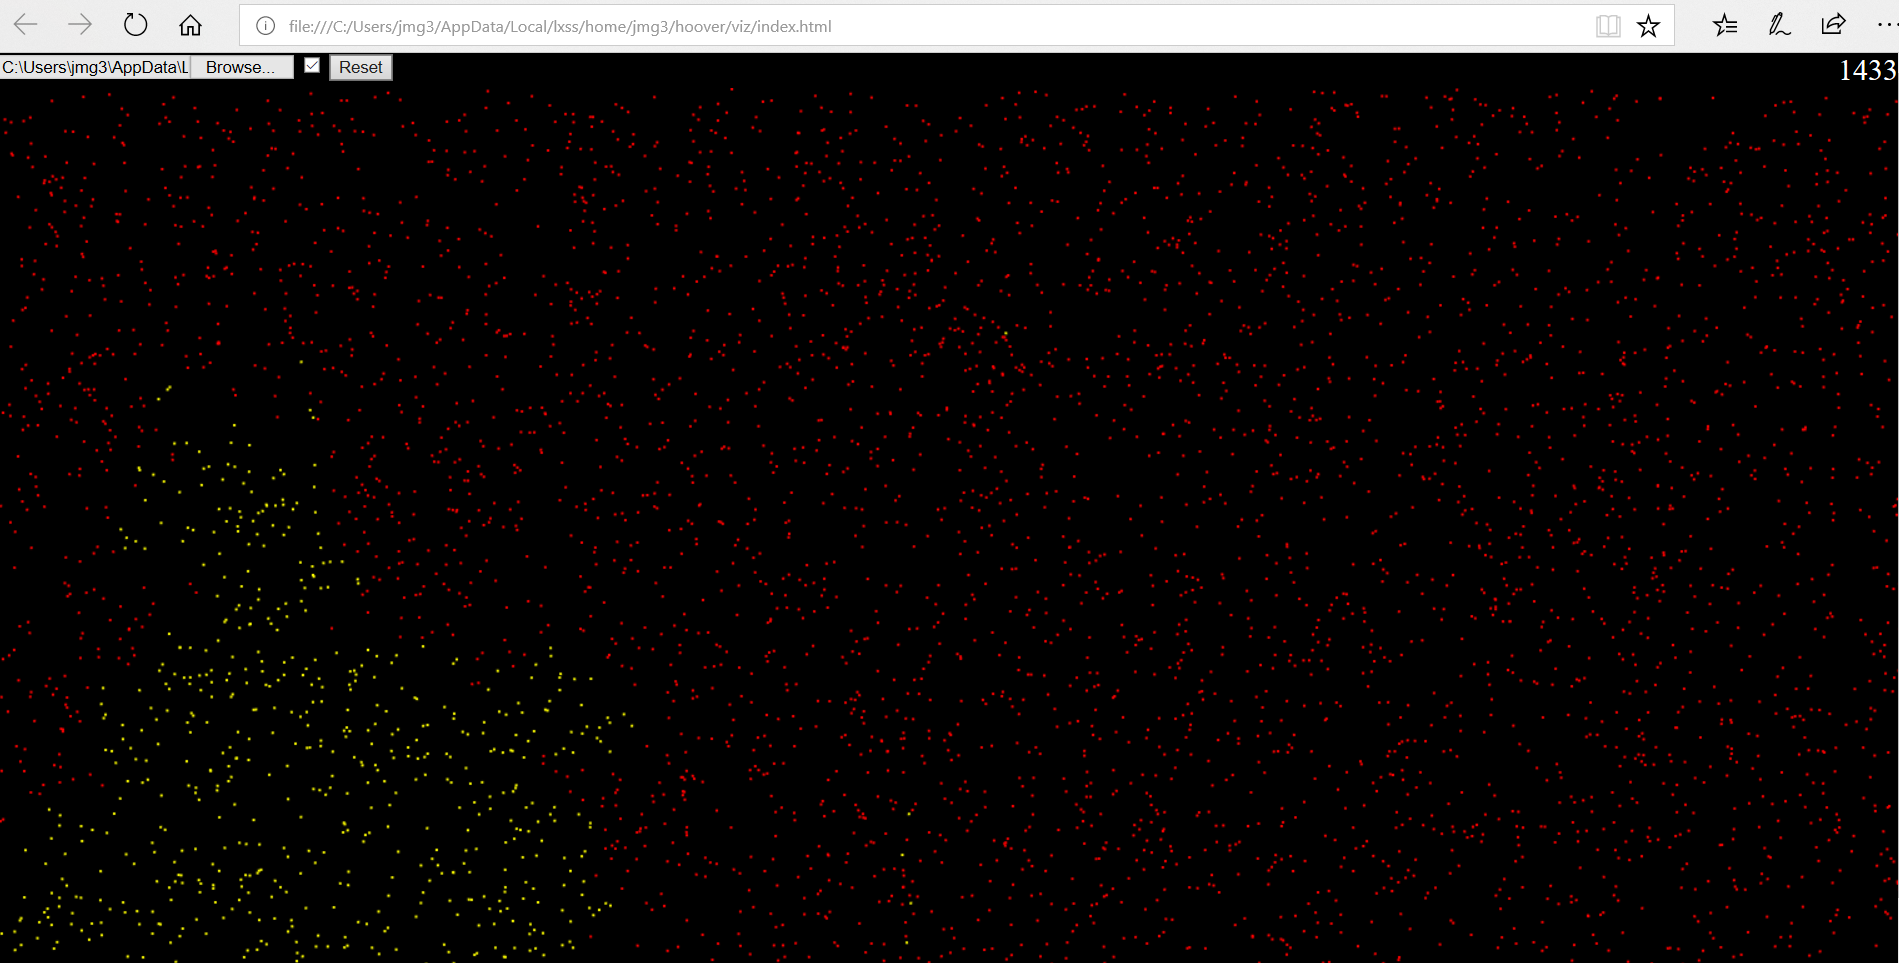
\includegraphics[width=\columnwidth]{hoover-viz.png}
\caption{Screenshot of the HOOVER-viz tool.}
\label{fig:hoover-viz}
\end{figure}


\section{Related Work}

STINGR

TODO

\section{Acknowledgements}

The authors would like to thank Steve Poole (LANL) for his valuable feedback on
the HOOVER project and this manuscript.

Work on HOOVER was funded in part by the United States Department of
Defense, and was supported by resources at Los Alamos National
Laboratory. This research used resources of the National Energy Research
Scientific Computing Center, a DOE Office of Science User Facility supported by
the Office of Science of the U.S. Department of Energy under Contract No. DE-AC02-05CH11231. This publication has been approved for public, unlimited distribution by Los
Alamos National Laboratory, with document number LA-UR-18-24291.


~\\
%\scriptsize
\bibliographystyle{splncs03}
%\bibliography{habanero}
\bibliography{paper}

\end{document}
